\documentclass[12pt,letterpaper]{article}
\usepackage{fullpage}
\usepackage[top=2cm, bottom=4.5cm, left=2.3cm, right=2.3cm]{geometry}
\usepackage{amsmath,amsthm,amsfonts,amssymb,amscd}
\usepackage{lastpage}
\usepackage{enumerate}
\usepackage{fancyhdr}
\usepackage{mathrsfs}
\usepackage{xcolor}
\usepackage{graphicx}
\usepackage{listings}
\usepackage{hyperref}

\hypersetup{%
  colorlinks=true,
  linkcolor=blue,
  linkbordercolor={0 0 1}
}
\usepackage{wrapfig}
\renewcommand\lstlistingname{Algorithm}
\renewcommand\lstlistlistingname{Algorithms}
\def\lstlistingautorefname{Alg.}

\lstdefinestyle{Python}{
    language        = Python,
    frame           = lines, 
    basicstyle      = \footnotesize
}

\setlength{\parindent}{0.0in}
\setlength{\parskip}{0.05in}

% Edit these as appropriate
\newcommand\course{CS 639}

%\pagestyle{fancyplain}
\headheight 35pt
\usepackage{xcolor}
% hyperref link defaults to "blue" (0000ff) as this matches our publisher produced pdf style
\definecolor{xlinkcolor}{cmyk}{1,1,0,0}
\usepackage{hyperref}
\fancypagestyle{firstpage}{
  \chead{\textbf{\Large  Bayesian vs Frequentist Approach \\in Medical Research \\}}
  \rhead{\course \\ \today}
  \lhead{ Harsh Sahu\\Lekshmi Thulasidharan }
  \lfoot{}
  \cfoot{}
  \rfoot{\small\thepage}
  \headsep 3em
}


\usepackage{amsmath}
\PassOptionsToPackage{hyphens}{url}
\fancypagestyle{normal}{
  %\renewcommand{\headrulewidth}{0.5pt}
  \headsep 3em
}

% Set the default page style to 'normal'
%\pagestyle{headings}
%\headsep 2em
%\fancyhead[R]{\rightmark}
%\renewcommand{\subsectionmark}[1]{\markright{#1}}

\pagestyle{headings}
\headsep 2em

%% In response to request from AAS 

\begin{document}
\par
%\thispagestyle{fancy}
\thispagestyle{firstpage}
\section{Introduction}
In medical research, statistical methods are commonly used to analyze data and draw conclusions. Two common approaches are the Bayesian and frequentist approaches. In simple words, Bayesian statistics involves the use of past/existing knowledge (a.k.a prior) along with the new data to make predictions, while frequentist statistics involves making inferences based on the observed data alone. We start this review with a comprehensive overview of each approach followed by a comparison study. Specifically, we try to answer the following questions:
\begin{itemize}
    \item What are the relative strengths and weaknesses of Bayesian and frequentist methods in the context of medical research?
    \item  Under which circumstances do the two approaches lead to similar or different conclusions?
    \item Does the use of one of these approaches increase the potential for breakthroughs in medical research compared to the other?
    \item What are the drawbacks of each approach?
\end{itemize}
We then review the application of Bayesian and frequentist methods in predicting the risk of dementia in older adults. 
\subsection{Frequentist Approach}
explain the foundations

\subsection{Bayesian Approach}
explain the foundations
\subsection{Comparison}
Also talk about medical research application. Case study : Dementia

\section{Application of frequentist approach in risk prediction of dementia in older adults}
Dementia is a common yet severe condition that primarily affects elder population. This is an umbrella term for conditions which could impair a person's ability to perform day to day activities since it has a detrimental effect on their cognition. For example, those who have dementia will experience memory loss, difficulty with communication and reasoning along with changes in psychological health. Unfortunately, there is currently no known cure for dementia. For this reason, it is extremely important to identify the individuals who are at very high risk for dementia early on, since this allows for incorporating lifestyle changes and treatments which could potentially slow the rate of progression of this condition. A straightforward method which allows the early identification of risk factors of dementia is by utilising statistical techniques to generate a risk score model. Researchers assign a score to every possible risk factors including demographic factors that could contribute to the development of dementia. Once we have the model, we can screen people and classify them into low, moderate and high risk populations. Within the frequentist approach, one statistical technique that can be highly effective in creating risk prediction models is the ``Logistic regression''. Here we review Barnes et al. (2009), where they developed one such risk score model i.e., a late life dementia index which can be used to accurately predict the chances of a person developing dementia in 6 years based on several risk factors using Logistic Regression. The tool they developed can be used to classify individuals into low, moderate and high risk categories for dementia, and hence serves as an excellent aid for monitoring vulnerable adults for dementia symptoms to start their treatment early on.  

\subsection{Logistic Regression}

\begin{wrapfigure}{r}{7cm}
\vspace{-7 mm}
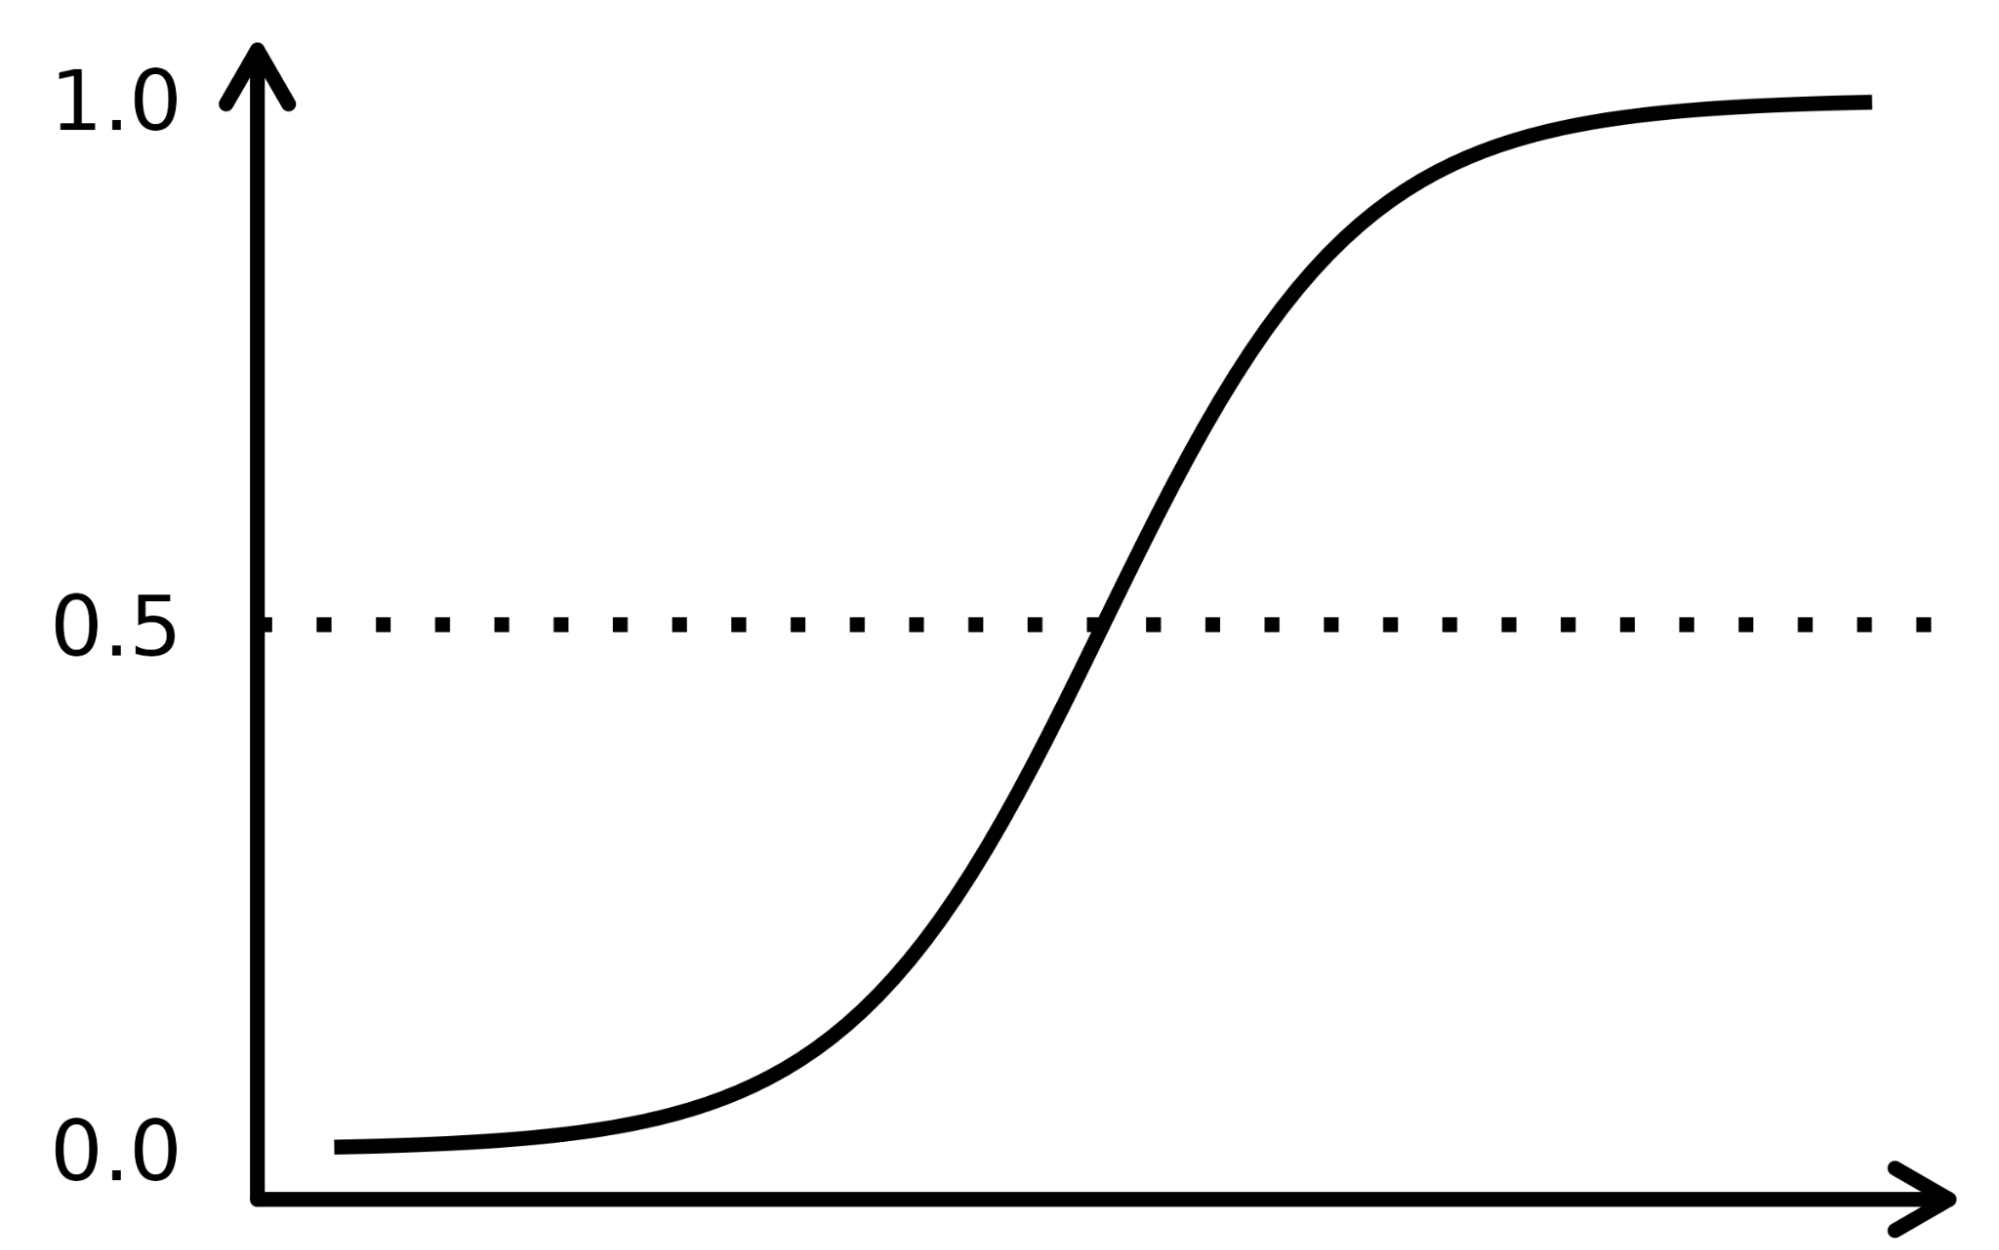
\includegraphics[width=7 cm]{sigmoid.png}
\caption{The sigmoid function curve}
\label{dvdr}
\end{wrapfigure}
Logistic Regression is a useful method for classification problems where we want to find the probability of a variable belongs to a particular category. So, this analysis is best for predicting binary outcomes like yes or no. In medical research this could translate into the probability of a patient developing a disease given one or more input variables (which would be the suspected risk factors). The probability is modelled using a logistic function which is a sigmoid (Fig.\ref{dvdr}) . The function takes a linear combination of the input variables and  and returns an output between 0 and 1. \\

When we have multiple input variables as in the case of risk prediction of a disease, the logistic function takes the form:
\begin{equation}
p(X) =Pr (Y|X)= \frac{e^{\beta_0+\beta_1X_1+\beta_2X_2+...+\beta_pX_p}}{1+e^{\beta_0+\beta_1X_1+\beta_2X_2+...+\beta_pX_p}}
\end{equation}

In the context of the paper we are discussing here, $Pr (Y|X)$ would the probability of a person developing dementia (modelled with variable $Y$) given certain risk factors (or predictors) assumed to be independent with each other($X=(X_1,X_2,\dots,X_p)$). The $\beta$ coefficients represent the parameters of the model, with $\beta_0$ being the intercept and $\beta_1,\beta_2,\dots,\beta_p$ being the coefficients for each of the independent variables. The coefficients can be estimated by maximizing the corresponding likelihood function.  

\subsection{Predictors of Dementia}

The data for different predictors were collected from the Cardiovascular Health Cognition Study which was started in 1989–1990 and updated during 1992–1993. They identified and classified individuals into three groups: (i) Those who already had dementia at the time of data collection, (ii) those who developed dementia after the data collection and (iii) those who developed mild cognitive impairment or MCI (this is not as severe as dementia) any time during the follow up period that lasted until 1998-1999. For this study, since the authors are interested in predicting the risk of dementia, they excluded individuals who belonged to the first category as well as those people who either died or lost contact before the follow up data is collected. This resulted in a sample size of 3,375. 

The authors consider a wide range of predictors for this study and they broadly belong to several categories described below:

(i) Demographic factors - This will help us understand if the risk of developing dementia is related to a person's age, gender, race, ethnicity, income etc.\\
(ii) Pre-exisitng medical conditions: Some of the medical conditions such as a history of stroke, diabetes etc. are known to increase the chances of a person developing dementia. \\
(iii)  Cognitive function : Cognitive function include a person's ability to learn, remember, reason, pay attention etc.  Since dementia is associated with a deterioration of cognitive abilities, this is a very important predictor of this condition. \\
(iv) Physical function measures: This is related to one's ability to perform normal day to day activities such as being able to get out of bed, eat, bath, walk, lift, carry weights etc without anyone's help. Since dementia is associated with weakened muscle strength and poor coordination, this is a very important risk factor. \\
(v) Physical performance measures: Some of the early symptoms of dementia involve taking more than usual time to perform certain normal activities. For eg. an individual could take more time to button or unbutton a shirt. So it is important to consider physical performance as a predictor.\\
(vi) Lifestyle factors: This involves information about one's alcohol consumption rate, smoking habits, time spent on exercise etc., which are indicators of how healthy a person is. \\
(vii) Psychosocial factors: This takes into consideration, a person's emotional and mental well-being. Authors make use of depression score, social network coverage of a person, how much support system a person has and the life events which could positively or negatively impact someone. \\
(viii) Cerebral MRI variables: Includes the presence of small or large tumors, white matter disease (damage to white matter of the brain usually associated with aging) etc. that could seriously affect a person's coordination.\\
(ix) Carotid artery ultrasound variables and Electrocardiogram measurements: Considering this could possibly unveil any correlation of dementia with one's cardiovascular health.\\
(x) Genetic factors: Studies have shown that the presence of APOE polymorphic alleles in the genes makes a person at the risk of Alzheimer disease which comes under dementia.\\
(xi) Serum measures: Certain blood tests could help understand the underlying condition that causes change in a person's ability to think, reason and remember. \\

This is in fact a lot of predictors. But not all of them will contribute to dementia equally. Some of them could be very good indicators whereas some won't have any effect at all. So before using Logistic Regression to evaluate the finalized logistic coefficients to develop a late life dementia risk score, it makes sense to eliminate some of these predictors from the analysis based on their statistical significance. To do this, careful and rigorous statistical analysis techniques should be used. In the next section, we will look into the methodology followed by the authors to choose the subset of relevant predictors.

\subsection{Methodology for Statistical Analysis}

Before doing any high level statistics to determine the relationship between predictor variables and the target variable (i.e. dementia) using the data of the former, we should always start simple. That is, first step should be to understand the observed data itself. For the entire sample size, we should start by  looking at the distribution of data for every single predictors. This is as simple as plotting a histogram which tells us about the frequency distribution of the variable under study along with its mean, median, range etc. Doing this will help us identify any outliers in the data and also help us quantify what ``high'' and ``low'' means for every variable. In other words, we can identify the cut off value for every variable above which the value of variable is too high and below which it is too low. This will aid us in categorization of individuals for every predictors. For eg. based on the distribution of age of the sample population used in the paper, range is from 65-100 years. A cut off was applied at 74 and 79 to divide the population into three groups- 65-74, 75-79 and 80-100. This is essential because some symptoms which are predictive of dementia could be simply a part of natural process of aging. So dividing the population based on age will help in removing any such biases and improve the accuracy of the analysis.\\

It is very important to categorize the variables before looking at their association with dementia. Doing this will not only make it easy to identify existing patterns but also make the data more interpretable by being able to visualize it better. For eg: one of the risk factors of dementia is poor physical performance when it comes to normal activities. A person who is under high risk of this disease might takes longer time to button a shirt compared to normal people.  Let's say the data of the time taken by a person to button a shirt consists of numbers ranging from 20 sec to 100 sec and the normal time to button a shirt is $\leq45$ sec. In this case, we can simply apply a cut off at $45$ sec and divide the data into two groups. We don't need to consider every data point and this makes it easier to study the associations, if any, with dementia. Categorization is a trivial thing to do when the variable we are considering is qualitative. For eg: Among the predictor variables that comes under demographic factors is the gender. It is essential to categorize individuals into biological male and female populations to study the association with dementia. 

\\



Once the univariate distribution of every risk factors in detail, authors looked at the bivariate distribution to explore the how these risk factors are related to dementia. To do this, $\chi^2$ test 




\end{document}
